\section{Architettura dell'applicazione}
\subsection{Descrizione generale}
L'architettura scelta per il \gl{sistema} dell'applicazione è quella a \gl{microservizi}.\\
I motivi che hanno spinto il \gl{team} a questa scelta sono stati i seguenti:
\begin{itemize}
	\item i servizi utilizzati di AWS permettono l'implementazione di un'architettura \gl{serverless}, la quale consente una migliore gestione dei microservizi, guadagnandone in facilità d'implementazione e di scalabilità di quest'ultimi;
	\item api.ai, il \gl{software} development kit (\gl{SDK}) scelto per la realizzazione dell'assistente virtuale, accetta in input solo del testo e non dell'audio, avendo così bisogno di un servizio differente e indipendente che, dato un file audio, estragga un testo corrisondente al suo contenuto;
	\item il \gl{proponente} ha richiesto anche un lato amministrazione, il quale accesso dovrà essere regolamentato da un servizio differente e indipendente di riconoscimento vocale.
\end{itemize}

Ogni microservizio rende disponibili degli \gl{endpoints}, tramite i quali è possibile lo scambio di dati. \\
Per poter creare, pubblicare, mantenere e monitorare le \gl{API} che consentono di usufruire delle funzionalità supportate dal back-end, è necessario realizzare un \gl{API Gateway} che si interpone tra client e back-end, permettendo al primo di comunicare con il secondo.
Esso permette inoltre la creazione di endpoint disponibili all'esterno del back-end, che verranno poi mappati negli endpoints supportati dal back-end, in particolare dai microservizi.\\
Allo stato attuale un solo tipo di client è supportato, ovvero quello vocale richiesto dal proponente.\\
Con lo scopo di semplificare al client l'uso del back-end, è stato deciso di rendere disponibile un solo endpoint esterno per il client. \\
I motivi che hanno spinto il team a questa scelta sono stati i seguenti:
\begin{itemize}
	\item dal punto di vista del client è molto più semplice fare utilizzo di un solo endpoint, demandando all'API Gateway la responsabilità di mappare la richiesta del client negli endpoints supportati dal backend;
	\item qualora si volesse aggiungere un client di tipo differente, ad esempio uno puramente testuale, sarà sufficiente pubblicare un nuovo endpoint esterno, mantenendo quindi semplice l'interfaccia dell'API Gateway;
	\item in caso ci siano dei cambiamenti nel back-end, la complessità del cambio di mappatura tra gli endpoint interni e l'endpoint esterno sarà contenuta in quest'ultimo;
\end{itemize}

In figura \ref{fig:apig1} si ha una rappresentazione generale, non specifica del \gl{progetto} \PROGETTO, del ruolo di un API Gateway in un'architettura a microservizi.\\

\begin{figure}[h]
	\centering
	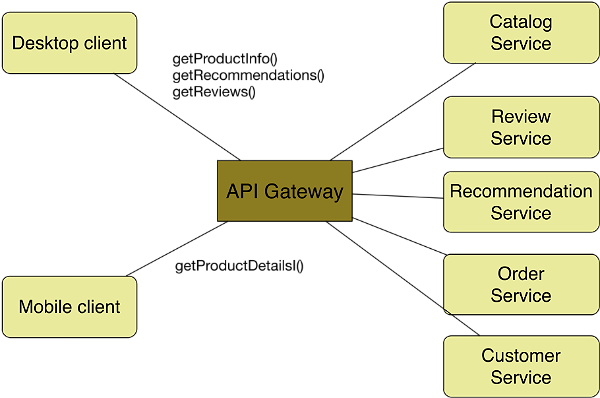
\includegraphics[width=\textwidth,height=\textheight,keepaspectratio,scale=0.1]{images/apigateway1.png}
	\caption{Architettura a microservizi e API Gateway}\label{fig:apig1}
\end{figure}
\newpage
Nella progettazione dell'architettura, il team ha seguito i vincoli posti dall'approccio architetturale \gl{REST}, i quali sono consultabili alla pagina \url{https://en.wikipedia.org/wiki/Representational_state_transfer} (visitato in data 2017-03-26).
\subsection{Sicurezza API Gateway ed endpoints}
Con lo scopo di garantire una certa sicurezza, l'accesso agli endpoints pubblicati sull'API Gateway deve essere controllato e regolato. \\Questo è necessario in quanto tramite essi è possibili fare operazioni sensibili sul sistema, quindi un utente malintenzionato potrebbe comprometterne il corretto funzionamento.\\ 
Il servizio AWS API Gateway fornisce sofisticati ed avanzati meccanismi per la protezione degli endpoint, i quali sono esposti e spiegati alla pagina \url{http://docs.aws.amazon.com/apigateway/latest/developerguide/permissions.html} (visitato in data 2017-03-26). \\

Il sistema progettato prevede due tipologie di utenti (ospite e amministratore), caratterizzati da diverse interazioni con l'assistente virtuale. Vengono quindi supportate dal \file{Back-end} differenti operazioni, invocabili tramite appositi endpoints, in base alla tipologia d'utente. Nasce di conseguenza la necessità di vincolare ogni tipologia d'utente ai soli endpoints ad essa dedicati. \\
Per soddisfare questa esigenza, non sono necessari ulteriori strumenti e meccanismi di AWS API Gateway, in quanto un amministratore è associato ad un \gl{JSON} Web Tokens (JWT) valido. Per capire quindi quali endpoints dovranno essere bloccati all'utente, sarà sufficiente controllare l'esistenza e la validità di questo JWT.
\subsection{Client}
\subsubsection{Client vocale}
L'architettura con la quale è organizzato il client vocale è quella \gl{event-driven}.\\
La motivazione che ha spinto il gruppo a prendere tale decisione è che ciò che dev'essere descritto e realizzato è facilmente modellabile utilizzando questo paradigma. Infatti, ci sono delle componenti che "aspettano" il verificarsi di un evento; altre invece che "notificano"  il verificarsi di un evento.\\
A tal fine, si è fatto utilizzo del pattern comportamentale \gl{Observer}.\\
Ad esempio, la componente \file{Recorder} (che si occupa della registrazione audio), deve prima "aspettare" che qualche individuo parli per potersi attivare, oppure deve "aspettare" che il riproduttore audio abbia terminato la riproduzione prima di potersi rimettere in ascolto.\\
Il client vocale è composto da diverse componenti, le quali sono:
\begin{itemize}
	\item \textbf{Recorder}: questa componente si occupa di realizzare le funzionalità di registrazione. Tramite la classe \file{Utility::BoolObserver}, facente parte del pattern comportamentale Observer utilizzato per modellare ciò, il registratore avrà modo di sapere se il riproduttore audio è in funzione, in maniera tale da non registrare le risposte fornite dal sistema. Una volta terminata la registrazione, il relativo audio verrà inviato alla componente \file{Logic};
	\newpage
	\item \textbf{TTS}: questa componente si occupa di realizzare le funzionalità di text-to-speech, ovvero di riprodurre sotto forma di audio il testo fornito come risposta dall'assistente virtuale. Inoltre, quando la riproduzione audio si attiva/disattiva, le componenti interessate vengono notificate di ciò. Tutto ciò è reso possibile dal pattern comportamentale Observer;
	\item \textbf{ApplicationManager}: questa componente si occupa realizzare le funzionalità di gestione delle applicazioni con le quali l'utente interagisce, permettendo la definizione di esse, la definizione comandi accettati, del salvataggio di stato e del cambio tra un'applicazione e l'altra. Tutto ciò è reso possibile dal pattern \gl{Client-side discovery} riadattato, la quale descrizione è consultabile nell'appendice \ref{CS}. Grazie all'utilizzo del pattern comportamentale Observer, questa componente viene notificata dell'arrivo di dati dal \file{Back-end};
	\item \textbf{ConversationApp}: questa componente si occupa di realizzare l'applicazione ConversationApp, ovvero quella che, tramite interfaccia utente, permette l'interazione con l'assistente virtuale. Per modellare la disposizione delle sue classi, si è fatto utilizzo del pattern Flux descritto nella libreria React, la quale verrà utilizzata per realizzare quanto appena descritto. 
	\item \textbf{Logic}: questa componente si occupa di realizzare le funzionalità che permettono l'interazione, tramite API Gateway, con il \file{Back-end}. Inoltre, quando arrivano dei dati da quest'ultimo, questa componente si occupa di notificare le componenti interessate. Ancora una volta, tutto ciò è organizzato secondo il pattern comportamentale Observer.
\end{itemize}
\subsubsection{Endpoints}
	Ora verranno definiti gli endpoints esterni utilizzati dai vari tipi di client.\\
	Per ogni risorsa sono stati specificati i formati per lo scambio dei dati in JSON:
	\begin{itemize}
		\item \textbf{Request:} rappresenta l’oggetto JSON che dovrà essere passato alla risorsa REST;
		\item \textbf{Response:} rappresenta l’oggetto JSON che fornirà in risposta la risorsa REST.
	\end{itemize}
	L'endpoint utilizzato dal client vocale è:
	\begin{itemize}
		\item \textbf{/query}\\
		\begin{itemize}
			\item \textbf{Method:} POST;
			\item \textbf{Descrizione:} invia all'API Gateway l'audio contenente la richiesta dell'utente;
			\item \textbf{Request:} la richiesta deve contenere i campi organizzati come descritto in \\\file{Back-end::APIGateway::VARequestAPIBody}:
\begin{lstlisting}[language=json,firstnumber=1]
{
 "app":"String",
 "audio":"Base64String",
 "data":"ObjectAssocArray",
 "session_id":"String"
}
\end{lstlisting}
			\item \textbf{Response:} la risposta deve contenere i campi organizzati come descritto in \\\file{Back-end::VirtualAssistant::VAResponse}:
\begin{lstlisting}[language=json,firstnumber=1]
{
"action":"String",
"res":{
 "contexts":"ObjectAssocArray",
 "data":"Object",
 "text_request":"String",
 "text_response":"String"
 },
"session_id":"String"
}
\end{lstlisting}
		\end{itemize}
	\end{itemize}

\subsection{Microservizi}
Di seguito verranno esposti e spiegati i funzionamenti di ogni microservizio da implementare.
\subsubsection{Virtual Assistant}
\paragraph{Descrizione}
Il microservizio Virtual Assistant (VA) fornisce le funzionalità di un assistente virtuale. Fa affidamento ad api.ai, e si occupa di inoltrare le richieste ricevute a tale infrastruttura. Avvalendosi di un database, permette di utilizzare diversi agenti (ciò che trasforma il linguaggio naturale in dati processabili per un'applicazione) durante la stessa interazione, consentendo quindi di definire diverse "applicazioni". Per ogni applicazione, si dovrà definire un agente.\\ Le richieste fatte all'unico endpoint di questo microservizio richiedono infatti di comunicare anche il nome dell'applicazione a cui è legata la richiesta. Questo permette di separare in diversi agenti di api.ai dialoghi legati a diverse funzionalità, affidando la realizzazione e l'integrazione di queste a diversi sviluppatori, senza dover modificare direttamente gli agenti di api.ai. \\
Per avere un completo controllo sul flusso della conversazione, si dovrà fare utilizzo di un database contenente gli agenti utilizzabili, in maniera tale che vengano usati solo quelli definiti e registrati.\\
Il microservizio si occupa anche di notificare, tramite l'utilizzo di AWS SNS, l'avvenuta interazione da parte dell'utente, permettendo così il salvataggio delle conversazioni in un database di supporto, il quale potrebbe essere utilizzato per fini di \gl{machine learning}.\\
Di seguito vengono esposti i vari passaggi affrontati all'arrivo di una richiesta:
\begin{itemize}
	\item arriva una richiesta;
	\item interrogo il database, contenente gli agenti, utilizzando il nome dell'applicazione come chiave;
	\item dall'interrogazione precedente ottengo il token dell'agente relativo all'applicazione;
	\item invio ad api.ai il token, e il testo della richiesta;
	\item api.ai fornisce la risposta, la quale viene "filtrata" da\\ \file{Back-end::VirtualAssistant::ApiAiVAAdapter::query(str: VAQuery): VAResponse}, ottenendo così un formato adatto a \file{Back-end::VirtualAssistant::VAResponse};
	\item pubblico, tramite il servizio Amazon SNS, la risposta filtrata che verrà quindi inviata al Client.
\end{itemize}
\paragraph{Endpoints}

Ora verranno definiti gli Endpoints utilizzati per i passaggi di risorse con il microservizio Virtual Assistant.\\
Per ogni risorsa sono stati specificati i formati per lo scambio dei dati in JSON:
\begin{itemize}
\item \textbf{Request:} rappresenta l’oggetto JSON che dovrà essere passato alla risorsa REST;
\item \textbf{Response:} rappresenta l’oggetto JSON che fornirà in risposta la risorsa REST.
\end{itemize}
Gli Endpoints sono:
\begin{itemize}
\item \textbf{/query}\\
\begin{itemize}
\item \textbf{Method:} POST;
\item \textbf{Descrizione:} invia al microservizio una richiesta per interrogare l'assistente virtuale;
\item \textbf{Request:} la richiesta deve contenere i campi organizzati come descritto in \\\file{Back-end::VirtualAssistant::VAQuery}:
\begin{lstlisting}[language=json,firstnumber=1]
{
 "data":"Object",
 "event":{ /*Alternativo a "text", oggetto di tipo VAEventObject*/
  "data":"Object",
  "name":"String"
 },
 "session_id":"String",
 "text":"String" /*Alternativo a "event"*/
}
\end{lstlisting}
\item \textbf{Response:} la risposta deve contenere i campi organizzati come descritto in \\\file{Back-end::VirtualAssistant::VAResponse}:
\begin{lstlisting}[language=json,firstnumber=1]
{
 "action":"String",
 "res":{/*oggetto di tipo ResponseBody*/
  "contexts":"ObjectAssocArray",
  "data":"Object",
  "text_request":"String",
  "text_response":"String"
 },
 "session_id":"String"
}
\end{lstlisting}
\end{itemize}
\end{itemize}


\subsubsection{Notifications}
\paragraph{Descrizione}
Il microservizio Notifications si occupa di mandare messaggi di notifica nei canali adeguati per notificare gli interessati dell'arrivo di un'ospite in azienda. Fornisce le API per richiedere la lista dei possibili destinatari, e per mandare il messaggio di notifica in un determinato canale. La lista dei canali viene restituita come un'array di stringhe, ognuna delle quali rappresenta un canale.\\
Il microservizio si occupa di interrogare le diverse liste fornite dalla piattaforma di messaggistica scelta e di combinarle in un'unica lista. Nel nostro caso, la piattaforma di messaggistica è \gl{Slack} e le diverse liste fornite riguardano utente, canali e gruppi privati. Quando si vuole mandare un messaggio, il campo \file{Back-end::Notifications::NotificationMessageEvent::send\_to} indica chi è il destinatario di tale messaggio.\\ \file{Back-end::Notifications::NotificationMessageEvent::msg} invece contiene il messaggio vero e proprio, nel formato definito dalla piattaforma di messaggistica su cui si appoggia il microservizio. Il formato utilizzato da Slack è consultabile alla pagina \url{https://api.slack.com/docs/message-buttons} (visitato in data 2017-03-26).
\paragraph{Endpoints}

Ora verranno definiti gli Endpoints utilizzati per i passaggi di risorse con il microservizio Notifications. \\
Per ogni risorsa sono stati specificati i formati per lo scambio dei dati in JSON:
\begin{itemize}
\item \textbf{Request:} rappresenta l’oggetto JSON che dovrà essere passato alla risorsa REST;
\item \textbf{Response:} rappresenta l’oggetto JSON che fornirà in risposta la risorsa REST.
\end{itemize}
Gli Endpoints sono:
\begin{itemize}

\item \textbf{/notifications}\\
\begin{itemize}
\item \textbf{Method:} GET;
\item \textbf{Descrizione:} restituisce la lista dei possibili canali destinatari;
\item \textbf{Response:} la risposta deve contenere i campi organizzati come descritto in \\\file{Back-end::Notifications::NotificationChannel}:
\begin{lstlisting}[language=json,firstnumber=1]
{
  "created": "String",
  "creator": "String",
  "id": "String",
  "is_archived": "boolean",
  "is_member": "boolean",
  "name": "String"
  "num_members": "int",
  "purpose": "Purpose",
  "topic": "Topic",
}
\end{lstlisting}
\end{itemize}

\begin{itemize}
\item \textbf{Method:} POST;
\item \textbf{Descrizione:} invia la notifica ad una determinata persona;
\item \textbf{Request:} la richiesta deve contenere i campi organizzati come descritto in \\\file{Back-end::Notifications::NotificationMsg}:
\begin{lstlisting}[language=json,firstnumber=1]
{
  "msg": [
	"attachments_array":[{},{}], /*Array di Back-end::Notifications::Attachment*/
	"response_type":"String",
	"text":"String"
	],
  "send_to": "String"
}
\end{lstlisting}
\end{itemize}
\end{itemize}

\subsubsection{Users}
\paragraph{Descrizione}
Il microservizio Users si occupa della gestione degli amministratori del nostro sistema. Esso fornisce delle API REST per modificare i dati relativi agli amministratori del nostro sistema presenti in un database. Viene integrato col servizio di Speech Recognition dall'API Gateway, per fornire la possibilità di effettuare il login, tramite impronta vocale, nel sistema.
\paragraph{Endpoints}

Ora verranno definiti gli Endpoints utilizzati per i passaggi di risorse con il microservizio Users. \\
Per ogni risorsa sono stati specificati i formati per lo scambio dei dati in JSON:
\begin{itemize}
\item \textbf{Request:} rappresenta l’oggetto JSON che dovrà essere passato alla risorsa REST;
\item \textbf{Response:} rappresenta l’oggetto JSON che fornirà in risposta la risorsa REST.
\end{itemize}

Gli Endpoints sono:

\begin{itemize}
\item \textbf{/auth/users}\\
\begin{itemize}
\item \textbf{Method:} GET;
\item \textbf{Descrizione:} restituisce la lista degli \file{User} presenti nel database;
\item \textbf{Response:} la risposta deve contenere un array contenente i campi organizzati come descritto in \\\file{Back-end::Auth::User}:
\begin{lstlisting}[language=json,firstnumber=1]
{
  user_array : [
  {
   "first_name":"String",
   "last_name":"String",
   "password":"String",
   "slack_channel":"String",
   "sr_id":"String",
   "username":"String"
  },
  {
   "first_name":"String",
   "last_name":"String",
   "password":"String",
   "slack_channel":"String",
   "sr_id":"String",
   "username":"String"
  },
  {
   "first_name":"String",
   "last_name":"String",
   "password":"String",
   "slack_channel":"String",
   "sr_id":"String",
   "username":"String"
  }
 ]
}
\end{lstlisting}
\end{itemize}

\begin{itemize}
\item \textbf{Method:} POST;
\item \textbf{Descrizione:} vengono inviati i dati necessari all'aggiunta di un nuovo \file{User} al database;
\item \textbf{Request:} la richiesta deve contenere i campi organizzati come descritto in\\ \file{Back-end::Auth::User}:
\begin{lstlisting}[language=json,firstnumber=1]
{
  "first_name":"String",
  "last_name":"String",
  "password":"String",
  "slack_channel":"String",
  "sr_id":"String",
  "username":"String"
}
\end{lstlisting}
\item \textbf{Response}: il corpo della risposta sarà vuoto, ma il risultato di questa operazione sarà comunque deducibile dal valore dello status code \gl{HTTP};
\end{itemize}

\item \textbf{/auth/users/:username}\\

\begin{itemize}
\item \textbf{Method:} PUT;
\item \textbf{Descrizione:} vengono modificati i dati dell'utente, il quale identificativo è specificato nel path, tramite sovrascrittura;
\item \textbf{Request:} la richiesta deve contenere i campi organizzati come descritto in \\\file{Back-end::Auth::User}
\begin{lstlisting}[language=json,firstnumber=1]
{
  "first_name":"String",
  "last_name":"String",
  "password":"String",
  "slack_channel":"String",
  "sr_id":"String",
  "username":"String"
}
\end{lstlisting}
\item \textbf{Response}: il corpo della risposta sarà vuoto, ma il risultato di questa operazione sarà comunque deducibile dal valore dello status code HTTP.
\end{itemize}

\begin{itemize}
\item \textbf{Method:} DELETE;
\item \textbf{Descrizione:} viene eliminato un utente, il quale identificativo è specificato nel path;
\item \textbf{Response}: il corpo della risposta sarà vuoto, ma il risultato di questa operazione sarà comunque deducibile dal valore dello status code HTTP;
\end{itemize}

\begin{itemize}
\item \textbf{Method:} GET;
\item \textbf{Descrizione:} vengono ricevuti i dati relativi ad un utente, il quale identificativo è specificato nel path;
\item \textbf{Response:} la risposta deve contenere i campi organizzati come descritto in \\\file{Back-end::Auth::User}:
\begin{lstlisting}[language=json,firstnumber=1]
{
  "first_name":"String",
  "last_name":"String",
  "password":"String",
  "slack_channel":"String",
  "sr_id":"String",
  "username":"String"
}
\end{lstlisting}
\end{itemize}

\end{itemize}

\subsubsection{Rules}
\paragraph{Descrizione}
Il microservizio Rules si occupa della gestione delle \gl{direttive} del sistema. Una direttiva è un'istruzione che viene data da un amministratore al sistema, la quale permette di modificare il comportamento del sistema stesso al verificarsi di certe condizioni. Tali condizioni possono essere legate alla persona che interagisce col sistema, la sua azienda di provenienza, oppure alla persona desiderata che viene richiesta.\\
Il sistema fornisce una serie di funzioni per modificare il suo comportamento, le quali indicano il modo in cui esso debba essere cambiato. \\
Una direttiva è costituita da:
\begin{itemize}
	\item una lista di target, che indica gli obiettivi (persone) ai quali deve essere applicata la direttiva;
	\item un'istanza di funzione, che indica quale delle funzioni disponibili deve essere applicata e, nel caso in cui tale funzione abbia dei parametri modificabili, con quali valori di quest'ultimi deve essere chiamata;
	\item un nome, il quale permette agli amministratori di identificare le diverse direttive;
	\item un id, il quale identifica univocamente la funzione all'interno del sistema;
	\item una flag di abilitazione, che permette di abilitare e disabilitare l'applicazione della direttiva da parte del sistema.
\end{itemize}

\paragraph{Endpoints}

Ora verranno definiti gli Endpoints utilizzati per i passaggi di risorse con il microservizio Rules.\\
Per ogni risorsa sono stati specificati i formati per lo scambio dei dati in JSON:
\begin{itemize}
\item \textbf{Request:} rappresenta l’oggetto JSON che dovrà essere passato alla risorsa REST;
\item \textbf{Response:} rappresenta l’oggetto JSON che fornirà in risposta la risorsa REST.
\end{itemize}
Gli Endpoints sono:

\begin{itemize}

\item \textbf{/impostazioni}\\

\begin{itemize}
\item \textbf{Method:} GET;
\item \textbf{Descrizione:} viene ricevuta la lista delle direttive;
\item \textbf{Response:} la risposta deve contenere un array contenente i campi organizzati come descritto in \\\file{Back-end::Rules::Rule}:
\begin{lstlisting}[language=json,firstnumber=1]
{
 rule_array : [
 {
  "ac_list":[
	"adm1":"String",
	"adm2":"String",
	...
   ],
  "ac_mode":"int",
  "enabled":"boolean",
  "id":"int",
  "name":"String",
  "targets":[ /*oggetti di tipo Back-end::Rules::RuleTarget*/
  {
   "company":"String",
   "member":"String",
   "name":"String"
  },
  {
   "company":"String",
   "member":"String",
   "name":"String"
  }
  ],
  "task":{ /* oggetto di tipo Back-end::Rules::RuleTaskInstance*/
   "params":{
	"par1":"Object",
	"par2":"Object",
	...
   }
   "task":"String"
  }
 }
 ]
}
\end{lstlisting}
\end{itemize}

\begin{itemize}
\item \textbf{Method:} POST;
\item \textbf{Descrizione:} viene creata una nuova direttiva;
\item \textbf{Request:} la richiesta deve contenere i campi organizzati come descritto in \\\file{Back-end::Rules::Rule}:
\begin{lstlisting}[language=json,firstnumber=1]
{
	rule : {
	  "ac_list":[
	    "adm1":"String",
	    "adm2":"String",
		...
	  ],
	  "ac_mode":"int",
	  "enabled":"boolean",
	  "id":"int",
	  "name":"String",
	  "targets":[ /* oggetti di tipo Back-end::Rules::RuleTarget */
	  {
		"company":"String",
		"member":"String",
		"name":"String"
      },
	  {
		"company":"String",
		"member":"String",
		"name":"String"
	  }
	  ],
	  "task":{ /* oggetto di tipo Back-end::Rules::RuleTaskInstance*/
		"params":{
		  "par1":"Object",
		  "par2":"Object",
		  ...
	   }
	  "task":"String"
	  }
	}
}
\end{lstlisting}
\item \textbf{Response}: il corpo della risposta sarà vuoto, ma il risultato di questa operazione sarà comunque deducibile dal valore dello status code HTTP;
\end{itemize}

\item \textbf{/impostazioni/:id}\\

\begin{itemize}
\item \textbf{Method:} PUT;
\item \textbf{Descrizione:} viene modificata una direttiva, il quale identificativo è specificato nel path, tramite sovrascrittura;
\item \textbf{Request:} la richiesta deve contenere i campi organizzati come descritto in \\\file{Back-end::Rules::Rule}:
\begin{lstlisting}[language=json,firstnumber=1]
{
  rule : {
	"ac_list":[
	 "adm1":"String",
	 "adm2":"String",
	...
    ],
	"ac_mode":"int",
	"enabled":"boolean",
	"id":"int",
	"name":"String",
	"targets":[ /* oggetti di tipo Back-end::Rules::RuleTarget */
	{
	 "company":"String",
	 "member":"String",
	 "name":"String"
	},
	{
	 "company":"String",
	 "member":"String",
	 "name":"String"
	}
	],
	"task":{ /* oggetto di tipo Back-end::Rules::RuleTaskInstance*/
	 "params":{
	  "par1":"Object",
	  "par2":"Object",
	  ...
	 }
	"task":"String"
   }
  }
}
\end{lstlisting}
\item \textbf{Response}: il corpo della risposta sarà vuoto, ma il risultato di questa operazione sarà comunque deducibile dal valore dello status code HTTP;
\end{itemize}

\begin{itemize}
\item \textbf{Method:} GET;
\item \textbf{Descrizione:} vengono richiesti dati relativi ad una specifica direttiva, il quale identificativo è specificato nel path;
\item \textbf{Response:} la risposta deve contenere i campi organizzati come descritto in \\\file{Back-end::Rules::Rule}:
\begin{lstlisting}[language=json,firstnumber=1]
{
	rule : {
	 "ac_list":[
	  "adm1":"String",
	  "adm2":"String",
	  ...
	  ],
	"ac_mode":"int",
	"enabled":"boolean",
	"id":"int",
	"name":"String",
	"targets":[ /* oggetti di tipo Back-end::Rules::RuleTarget */
	{
	 "company":"String",
	 "member":"String",
	 "name":"String"
	},
	{
	 "company":"String",
	 "member":"String",
	 "name":"String"
	}
	],
	"task":{ /* oggetto di tipo Back-end::Rules::RuleTaskInstance*/
	 "params":{
	  "par1":"Object",
	  "par2":"Object",
	  ...
	 }
	"task":"String"
	}
  }
}
\end{lstlisting}

\end{itemize}

\begin{itemize}
\item \textbf{Method:} DELETE;
\item \textbf{Descrizione:} viene eliminata una direttiva, il quale identificativo è specificato nel path;
\item \textbf{Response}: il corpo della risposta sarà vuoto, ma il risultato di questa operazione sarà comunque deducibile dal valore dello status code HTTP;
\end{itemize}


\item \textbf{/impostazioni/tasks}\\

\begin{itemize}
\item \textbf{Method:} GET;
\item \textbf{Descrizione:} viene richiesta la lista dei tipi di funzioni presenti nel sistema;
\item \textbf{Response:} la risposta deve contenere i campi organizzati come descritto in \\\file{Back-end::Rules::Task}:
\begin{lstlisting}[language=json,firstnumber=1]
{
 function_array : [
 {
  "function":"String",
  "id":"int"
 },
 {
  "function":"String",
  "id":"int"
 }
]
}
\end{lstlisting}
\end{itemize}

\begin{itemize}
\item \textbf{Method:} POST;
\item \textbf{Descrizione:} viene creato un nuovo tipo di \file{Task};
\item \textbf{Request:} la richiesta deve contenere i campi organizzati come descritto in \\\file{Back-end::Rules::Task}:
\begin{lstlisting}[language=json,firstnumber=1]
{
 function_array : [
 {
  "function":"String",
  "id":"int"
 },
 {
  "function":"String",
  "id":"int"
 }
 ]
}
\end{lstlisting}
\item \textbf{Response}: il corpo della risposta sarà vuoto, ma il risultato di questa operazione sarà comunque deducibile dal valore dello status code HTTP.
\end{itemize}



\item \textbf{/impostazioni/tasks/:type}\\

\begin{itemize}
\item \textbf{Method:} GET;
\item \textbf{Descrizione:} viene richiesto un \file{Task} in base al tipo di funzione applicata, , il quale identificativo è specificato nel path;

\item \textbf{Response:} la risposta deve contenere i campi organizzati come descritto in \\\file{Back-end::Rules::Task}:
\begin{lstlisting}[language=json,firstnumber=1]
{
 function_array : [
 {
  "function":"String",
  "id":"int"
 },
 {
  "function":"String",
  "id":"int"
 }
 ]
}
\end{lstlisting}
\end{itemize}

\begin{itemize}
\item \textbf{Method:} PUT;
\item \textbf{Descrizione:} viene modificata un \file{Task}, il quale identificativo è specificato nel path tramite sovrascrittura;
\item \textbf{Request:} la richiesta deve contenere i campi organizzati come descritto in \\\file{Back-end::Rules::Task}:
\begin{lstlisting}[language=json,firstnumber=1]
{
 function_array : [
 {
  "function":"String",
  "id":"int"
 },
 {
  "function":"String",
  "id":"int"
 }
 ]
}
\end{lstlisting}
\item \textbf{Response}: il corpo della risposta sarà vuoto, ma il risultato di questa operazione sarà comunque deducibile dal valore dello status code HTTP.
\end{itemize}

\end{itemize}
\newpage
\subsection{Action supportate} \label{action}
Di seguito vengono elencate le action, supportate dal \file{Back-end}, che api.ai può ritornare in seguito alla richiesta di un utente. \\
Una action è una stringa che indica quale operazione dovrà essere scelta dall'API Gateway, in modo da soddisfare le richieste dell'utente.\\
I metodi citati appartengono alla classe \file{Back-end::APIGateway::VocalAPI}.
\subsubsection{User}
\begin{itemize}
\item \file{user.add}: utilizza il metodo privato \file{addUser(user: User)} per aggiungere un utente registrato, cioè un amministratore, al sistema;

\item \file{user.get}: utilizza il metodo privato \file{getUser(username: String)} per ottenere i dati relativi ad un utente registrato;

\item \file{user.getList}: utilizza il metodo privato \file{getUserList()} per ottenere la lista degli utenti registrati; 

\item \file{user.update}: utilizza il metodo privato \file{updateUser(user: User)} per aggiornare un utente registrato;

\item \file{user.remove}: utilizza il metodo privato \file{removeUser(username: String)} per rimuovere un utente registrato;

\item \file{user.addEnrollment}: utilizza il metodo privato \file{addUserEnrollment(enr: Enrollment)} per aggiungere un Enrollment ad un utente registrato;

\item \file{user.resetEnrollments}: utilizza il metodo privato \file{resetUserEnrollment(username: String):} per resettare gli Enrollment relativi ad un utente registrato;

\item \file{user.login}: utilizza il metodo privato \file{loginUser(enr: Enrollment)} per effettura il login di un utente registrato.

\end{itemize}
\subsubsection{Rule}
\begin{itemize}
\item \file{rule.add}: utilizza il metodo privato \file{addRule(rule: Rule)} per aggiungere una direttiva;

\item \file{rule.get}: utilizza il metodo privato \file{getRule(id: String)} per ottenere i dati relativi una direttiva;

\item \file{rule.getList}: utilizza il metodo privato \file{getRuleList()} per ottenere la lista delle direttive;

\item \file{rule.update}: utilizza il metodo privato \file{updateRule(rule: Rule)} per aggiornare una direttiva;

\item \file{rule.remove}: utilizza il metodo privato \file{removeRule(id: String)} per rimuovere una direttiva.


\end{itemize}
